\chapter{Introdução}\label{cap:introducao}



A navegação visual de veículos aéreos não tripulados (UAVs, do inglês \emph{unmanned aerial vehicles}) depende da capacidade de transformar imagens em informações úteis sobre o ambiente. Uma câmera monocular tem baixo peso e custo, mas não fornece diretamente a distância dos obstáculos. Essa informação precisa ser inferida a partir da aparência da cena, do movimento observado ou de modelos de aprendizado de máquina para estimar profundidade da cena. Mesmo com os avanços da estimação monocular de profundidade, erros de escala, oclusões e diferenças entre os dados de treinamento e o ambiente de uso continuam relevantes para aplicações em robótica \cite{Vyas2022,Arampatzakis2024,DepthAnythingV2}.

O desempenho de um sistema de navegação também depende da relação entre percepção, planejamento e execução do voo \cite{Loquercio2021}. Uma imagem contém muitos pixels. Um obstáculo fino ocupa poucos deles, de modo que seu erro pode ser alto mesmo quando a média global é baixa. Uma distância superestimada pode indicar uma passagem inexistente no mapa. Nesse caso, a estimativa pode atender a um critério numérico de profundidade e ainda representar um obstáculo como espaço livre. Por isso, interessa avaliar tanto a qualidade da estimativa quanto as consequências de seu uso em um mapa de ocupação.

Este trabalho adota a perspectiva de investigar os dados antes de aumentar a complexidade da arquitetura. O desenvolvimento começou com um fluxo reativo que gerou trajetórias e imagens da câmera, deslocamentos aparentes entre quadros e medições do giroscópio e do acelerômetro. A partir desses registros, o foco passou para a organização dos sinais, a análise dos erros e a comparação controlada de modelos. Em uma segunda etapa, a investigação incorporou mapeamento tridimensional e planejamento com A* \cite{Hart1968}, para verificar se a profundidade estimada produzia informação espacial utilizável.

\section{Problema e posição defendida}

A questão central é como avaliar a informação visual e inercial antes de empregá-la na tomada de decisão de um UAV. Essa avaliação envolve a sincronização dos sinais, a separação dos dados de treinamento e avaliação, a estabilidade dos modelos e a localização das falhas. A divisão por execução merece atenção porque amostras vizinhas de uma mesma trajetória podem compartilhar condições muito semelhantes e favorecer estimativas otimistas de generalização \cite{Kapoor2023}.

Este trabalho defende que a aprovação por métricas de profundidade deve ser acompanhada de evidência sobre ocupação e caminhos antes da integração de um estimador monocular ao voo. A recomendação permite usar métricas por pixel na seleção inicial, mas exige verificar também falso espaço livre, disponibilidade de planejamento e interseção dos caminhos com a referência.

Trabalhos sobre navegação visual combinam estimação de profundidade, representação do ambiente e planejamento \cite{Pan2024MoNA,Simon2024MonoNav}. Este estudo examina a passagem entre essas etapas para verificar os efeitos dos erros de percepção no mapa e nos caminhos. A proposta de \textit{Antes da Arquitetura} é usar a análise dos dados e dos erros para orientar mudanças no sistema.

Sementes aleatórias controlam a inicialização dos pesos e outras operações aleatórias do treinamento. Na análise tabular, eventos indicam mudanças de proximidade acima do limiar adotado. A classificação identifica sua ocorrência, enquanto a regressão estima sinal e magnitude. Ablação consiste em retirar um grupo de entradas e repetir a avaliação. A etapa de validação espacial reúne critérios de quantidade de quadros, disponibilidade de planejamento, falso espaço livre e colisão discreta, sem constituir certificação de segurança.

O percurso contém superfícies do solo, troncos e copas, com espaços abertos e trechos parcialmente encobertos. A Figura~\ref{fig:contexto-revisado} apresenta instantes do mesmo registro para situar essa variação visual, sem afirmar que os quadros constituem avaliação de iluminação ou cenários independentes.

\begin{figure}[htbp]
\centering
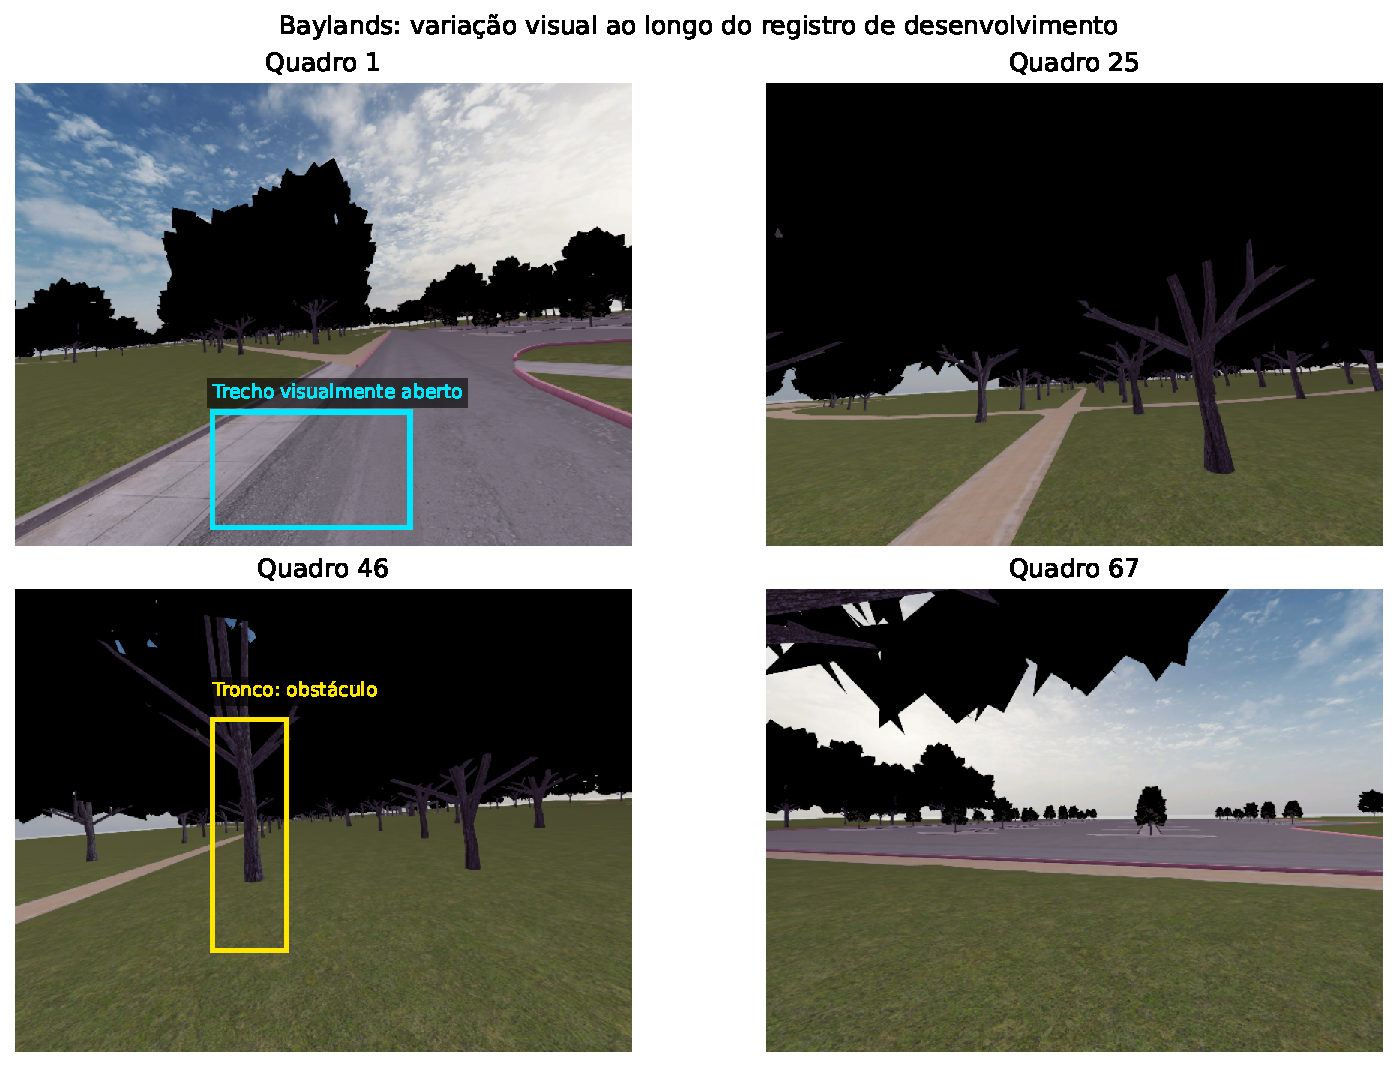
\includegraphics[width=.95\linewidth]{figuras/metodologia_cenas_contexto.pdf}
\caption{Quadros 1, 25, 46 e 67 do registro de desenvolvimento utilizado no replay monocular final. São imagens reais do simulador. As marcações manuais destacam um trecho visualmente aberto e um tronco, sem detecção semântica automática ou certificação de espaço livre.}
\label{fig:contexto-revisado}
\end{figure}

\section{Perguntas de pesquisa}

O estudo foi organizado em torno das seguintes perguntas:

\begin{enumerate}
    \item O aumento do número de execuções melhora a previsão das mudanças de proximidade?
    \item Os resultados permanecem estáveis entre sementes e diante de modelos de referência?
    \item Quais grupos de entradas mais contribuem para a generalização e para a interpretação dos erros?
    \item Separar a detecção de eventos da regressão ajuda a identificar onde o erro de proximidade se concentra?
    \item Uma estimativa monocular aprovada por métricas de profundidade também permite construir caminhos espaciais seguros?
\end{enumerate}

\section{Objetivos}

Os objetivos orientam a organização dos sinais e a avaliação espacial antes da integração ao voo.

\subsection{Objetivo geral}

Desenvolver e aplicar um protocolo documentado de avaliação visual e inercial de um UAV, reunindo diagnósticos por intervalos sincronizados e avaliação espacial da profundidade para discutir critérios de integração ao voo.

\subsection{Objetivos específicos}

Os objetivos específicos são:

\begin{itemize}
    \item organizar sinais de diferentes fontes em intervalos visuais e preservar a separação por execução;
    \item avaliar o crescimento do conjunto de treinamento com validação e teste fixos;
    \item comparar um perceptron multicamada (MLP \cite{Rumelhart1986}) com referências constantes e modelos de árvores, considerando diferentes sementes;
    \item investigar eventos de proximidade, sensibilidade por gradientes e ablação dos grupos de entradas;
    \item construir mapas de ocupação e aplicar A* com verificações de segurança;
    \item validar a geometria e o planejamento com profundidade de referência do simulador;
    \item avaliar a profundidade monocular por critérios por pixel e espaciais antes de sua integração ao voo.
\end{itemize}

\section{Visão geral e escopo}

O PX4 é o piloto automático, o Gazebo simula veículo e ambiente, e o ROS~2 realiza a comunicação entre componentes. O primeiro eixo reúne 40 execuções e 1.234 intervalos válidos, nos quais variações de sinais visuais, inerciais, de movimento e de comandos são relacionadas a variações de proximidade. O segundo eixo utiliza subconjuntos documentados de 103 diretórios de execuções espaciais completas, produzidas em etapas distintas de desenvolvimento, treinamento, diagnóstico e validação. Esses dois conjuntos possuem finalidades diferentes e não formam uma única bateria de repetições equivalentes.

No eixo espacial, a profundidade do Gazebo fornece a referência e também alimenta a bateria de validação da geometria e do planejamento. A alternativa monocular parte das imagens RGB e de uma variante métrica do Depth Anything V2 ajustada ao cenário \cite{DepthAnythingV2}. A avaliação offline verifica a profundidade, a ocupação e os caminhos antes de autorizar experimentos integrados ao voo.

O recorte não inclui o desenvolvimento de leis de controle nem sua comparação. O fluxo espacial substitui a decisão reativa de desvio por mapa e A*, enquanto o PX4 mantém a estabilização e o acompanhamento dos pontos de passagem. O fluxo reativo anterior permanece separado para continuidade futura. A investigação considera obstáculos estáticos em simulação e não demonstra prontidão para voo real ou desvio de objetos móveis.

Este trabalho apresenta alinhamento com o Objetivo de Desenvolvimento Sustentável 9 (ODS~9), relacionado à indústria, à inovação e à infraestrutura, em particular com a dimensão de fortalecimento da pesquisa científica e das capacidades tecnológicas da meta~9.5 da Agenda~2030 \cite{ONUAgenda2030}. A contribuição consiste na avaliação documentada de métodos de percepção e planejamento para veículos aéreos não tripulados e na disponibilização de código e resultados para reprodução. Esse alinhamento é tecnológico e metodológico. O estudo não mensurou benefícios ambientais, sociais ou econômicos decorrentes de sua aplicação.

\section{Contribuições do estudo}

O trabalho reúne a análise dos sinais sincronizados, a comparação entre modelos e sementes e a avaliação da profundidade no mapa e no planejador. O código permite repetir as decisões a partir dos registros e verificar por que uma configuração foi aceita ou rejeitada. A principal contribuição é o estudo dessas relações no cenário avaliado, incluindo os casos em que atender aos critérios por pixel não bastou para aprovar a utilização espacial.

Os eixos tabular e espacial utilizam conjuntos e objetivos diferentes. Os achados sobre entradas tabulares não foram transferidos e testados como melhorias do estimador denso.

\section{Organização do texto}\label{Organizacao_do_texto}

O Capítulo~\ref{cap:fundamentacao} apresenta a fundamentação teórica. O Capítulo~\ref{cap:relacionados} discute os trabalhos relacionados. O Capítulo~\ref{cap:proposta} define a proposta metodológica, e o Capítulo~\ref{cap:implementacao} descreve sua implementação. O Capítulo~\ref{cap:validacao} reúne os experimentos e os resultados. O Capítulo~\ref{cap:conclusoes} responde às perguntas de pesquisa e discute as contribuições, as limitações e as possibilidades de continuidade.
